\documentclass[11pt,a4paper]{article}

\usepackage[utf8]{inputenc}
\usepackage[T1]{fontenc}
\usepackage{lmodern}
\usepackage[margin=2.2cm]{geometry}
\usepackage{graphicx}
\usepackage{booktabs}
\usepackage{tabularx}
\usepackage{longtable}
\usepackage{array}
\usepackage{xcolor}
\usepackage{hyperref}
\usepackage{listings}
\usepackage{enumitem}
\usepackage{fancyhdr}
\usepackage{titlesec}
\usepackage{tikz}
\usetikzlibrary{shapes.geometric, arrows.meta, positioning, fit, backgrounds}

% Colors
\definecolor{primary}{HTML}{1B4F72}
\definecolor{secondary}{HTML}{2874A6}
\definecolor{accent}{HTML}{1E8449}
\definecolor{alertred}{HTML}{C0392B}
\definecolor{codebg}{HTML}{F4F6F7}
\definecolor{bordergray}{HTML}{D5DBDB}

\hypersetup{
    colorlinks=true,
    linkcolor=primary,
    urlcolor=secondary,
    pdftitle={Emporio da Musica - AI Customer Service Agent Documentation},
    pdfauthor={Flavio Midea}
}

% Header and Footer
\pagestyle{fancy}
\fancyhf{}
\fancyhead[L]{\small\textcolor{gray}{Emp\'orio da M\'usica --- AI Engineer Technical Challenge (Artefact)}}
\fancyhead[R]{\small\textcolor{gray}{Project README \& Technical Documentation}}
\fancyfoot[C]{\small\thepage}
\renewcommand{\headrulewidth}{0.4pt}

% Section styling
\titleformat{\section}{\Large\bfseries\color{primary}}{\thesection.}{0.5em}{}[\titlerule]
\titleformat{\subsection}{\large\bfseries\color{secondary}}{\thesubsection}{0.5em}{}

% Code listings style
\lstset{
    backgroundcolor=\color{codebg},
    basicstyle=\ttfamily\footnotesize,
    breaklines=true,
    frame=single,
    rulecolor=\color{bordergray},
    showstringspaces=false,
    tabsize=2,
    literate={á}{{\'a}}1 {ã}{{\~a}}1 {â}{{\^a}}1 {à}{{\`a}}1
             {é}{{\'e}}1 {ê}{{\^e}}1 {í}{{\'i}}1 {ó}{{\'o}}1
             {õ}{{\~o}}1 {ô}{{\^o}}1 {ú}{{\'u}}1 {ç}{{\c{c}}}1
             {Á}{{\'A}}1 {Ã}{{\~A}}1 {É}{{\'E}}1 {Í}{{\'I}}1
             {Ó}{{\'O}}1 {Õ}{{\~O}}1 {Ú}{{\'U}}1 {Ç}{{\c{C}}}1
             {º}{{\textordmasculine}}1 {—}{{---}}1 {–}{{--}}1
}

\setlength{\parskip}{0.45em}
\setlength{\parindent}{0pt}
\setlength{\emergencystretch}{3em}
\setlist[itemize]{noitemsep, topsep=2pt}
\setlist[enumerate]{noitemsep, topsep=2pt}

% Helper for breakable inline code
\newcommand{\code}[1]{\texttt{\seqsplit{#1}}}

\begin{document}

% ------------------------------------------------------------------ TITLE
\begin{center}
    {\LARGE\bfseries\color{primary} Emp\'orio da M\'usica --- Customer Service AI Agent}\\[0.4em]
    {\large\bfseries Technical Challenge --- AI Engineer (Artefact)}\\[0.3em]
    {\normalsize Project README \& Technical Documentation}\\[0.5em]
    {\small\textbf{Author:} Flavio Midea \quad|\quad \textbf{Stack:} Python $\cdot$ LangChain $\cdot$ MCP $\cdot$ Ollama (\texttt{qwen3.5:4b}) $\cdot$ SQLite $\cdot$ Streamlit}
\end{center}
\vspace{0.3em}
\hrule
\vspace{0.8em}

% ------------------------------------------------------------------ 1. OVERVIEW
\section{Project Overview}

This repository contains a functional prototype of a text-messaging customer-service AI agent built for \textbf{Emp\'orio da M\'usica}, a fictional musical instrument store located in Campo Grande/MS, Brazil (\textit{``Sua m\'usica come\c{c}a aqui''}), developed for the Artefact AI Engineer Technical Challenge.

The store's support team is overloaded with recurring questions regarding opening hours, order status, product prices, stock availability, promotions, and return/warranty policies. Our agent (\textbf{L\'eo}) runs \textbf{100\% locally via Ollama}, queries operational data and official policies through a decoupled \textbf{Model Context Protocol (MCP) server}, and enforces deterministic business rules in Python/SQLite.

By default, the agent handles customer conversations autonomously. Whenever it faces an out-of-policy request, a formal complaint, an action it is not allowed to execute (such as processing a return or cancelling an order), or missing information, it \textbf{escalates the conversation to a human attendant}, triggering a \textcolor{alertred}{\textbf{RED alert}} on the shopkeeper's dashboard and remaining silent on that thread until the shopkeeper returns control to the AI.

\begin{quote}
\textbf{Note (Prototype Scope):} The user interface is built in \textbf{Streamlit} to simulate both the customer's WhatsApp view and the shopkeeper's management dashboard in a single self-contained prototype. It is not connected to the live WhatsApp Business API (see Section~\ref{sec:limitations}).
\end{quote}

% ------------------------------------------------------------------ 2. ARCHITECTURE
\section{System Architecture \& How It Works}

\begin{center}
\resizebox{0.96\textwidth}{!}{%
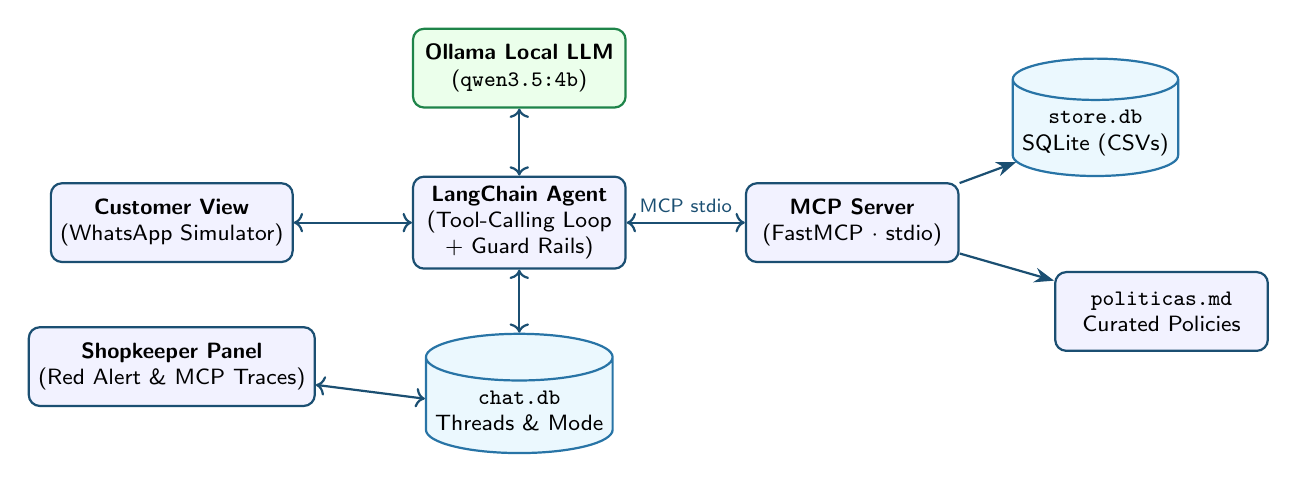
\begin{tikzpicture}[
    node distance=1.0cm and 1.3cm,
    box/.style={rectangle, rounded corners=4pt, draw=primary, fill=blue!5, thick, minimum height=1.0cm, minimum width=2.7cm, align=center, font=\footnotesize\sffamily},
    db/.style={cylinder, shape border rotate=90, aspect=0.25, draw=secondary, fill=cyan!8, thick, minimum height=1.05cm, minimum width=2.1cm, align=center, font=\footnotesize\sffamily},
    llm/.style={rectangle, rounded corners=4pt, draw=accent, fill=green!8, thick, minimum height=1.0cm, minimum width=2.7cm, align=center, font=\footnotesize\sffamily},
    arrow/.style={-{Stealth[length=2.5mm]}, thick, color=primary}
]
    \node[box] (client) {\textbf{Customer View}\\(WhatsApp Simulator)};
    \node[box, below=0.8cm of client] (shop) {\textbf{Shopkeeper Panel}\\(Red Alert \& MCP Traces)};
    \node[box, right=1.5cm of client] (agent) {\textbf{LangChain Agent}\\(Tool-Calling Loop\\+ Guard Rails)};
    \node[llm, above=0.85cm of agent] (ollama) {\textbf{Ollama Local LLM}\\(\texttt{qwen3.5:4b})};
    \node[box, right=1.5cm of agent] (mcp) {\textbf{MCP Server}\\(FastMCP $\cdot$ stdio)};
    \node[db, above right=0.1cm and 1.2cm of mcp] (storedb) {\textbf{\texttt{store.db}}\\SQLite (CSVs)};
    \node[box, below right=0.1cm and 1.2cm of mcp] (pol) {\textbf{\texttt{politicas.md}}\\Curated Policies};
    \node[db, below=0.8cm of agent] (chatdb) {\textbf{\texttt{chat.db}}\\Threads \& Mode};

    \draw[arrow, <->] (client) -- (agent);
    \draw[arrow, <->] (agent) -- (ollama);
    \draw[arrow, <->] (agent) -- node[above, font=\scriptsize\sffamily]{MCP stdio} (mcp);
    \draw[arrow] (mcp) -- (storedb);
    \draw[arrow] (mcp) -- (pol);
    \draw[arrow, <->] (agent) -- (chatdb);
    \draw[arrow, <->] (shop) -- (chatdb);
\end{tikzpicture}%
}
\end{center}

\subsection{MCP Tools Exposed (\texttt{app/mcp\_server/server.py})}

\begin{tabularx}{\textwidth}{>{\ttfamily\footnotesize\raggedright\arraybackslash}p{3.6cm} >{\raggedright\arraybackslash}X}
\toprule
\textbf{\normalfont\bfseries Tool Name} & \textbf{Purpose \& When the Agent Calls It} \\
\midrule
search\_products & Searches the catalog with exact filters (\texttt{query}, \texttt{max\_price}, \texttt{min\_price}, \texttt{only\_available}, \texttt{on\_promotion}). Used for budget queries (e.g., ``guitars up to R\$ 1000'') or active promotions. \\
\addlinespace[2pt]
get\_product\_details & Fetches full specs, original/promotional price, PIX price (5\% discount, non-cumulative with active promos), max interest-free installments, stock status, and automatic similar alternatives if out-of-stock or discontinued. \\
\addlinespace[2pt]
list\_categories & Lists all 9 musical instrument categories sold by the store with active product counts. \\
\addlinespace[2pt]
get\_customer\_orders & Retrieves orders belonging \textbf{exclusively to the current customer}, including status, items, tracking code, cancellation notes, and precomputed return/warranty eligibility (\texttt{policy\_check}). \\
\addlinespace[2pt]
get\_store\_policies & Deterministic topic-based retrieval of the store manual (\texttt{about\_and\_contact}, \texttt{opening\_hours}, \texttt{payment}, \texttt{returns\_exchanges}, \texttt{shipping}, \texttt{promotions}, \texttt{special\_situations}, \texttt{warranty}, \texttt{privacy}). \\
\addlinespace[2pt]
get\_opening\_status & Checks in real time whether the store is open right now, today's hours, and the next opening time. \\
\bottomrule
\end{tabularx}

In addition, the agent has a local tool \texttt{request\_human\_handoff(reason)} (kept outside the read-only MCP server because it mutates conversation state in \texttt{chat.db}).

\subsection{Human-in-the-Loop Escalation Lifecycle}
Each customer thread in \texttt{chat.db} has a \texttt{mode} state machine:
\begin{enumerate}
    \item \texttt{agent} (\textbf{Green --- Default}): The AI agent answers customer messages autonomously.
    \item \texttt{waiting\_human} (\textbf{\textcolor{alertred}{Red Alert}}): Triggered when the agent calls \texttt{request\_human\_handoff} (or via safety guard rails). A prominent red banner appears at the top of the shopkeeper's dashboard showing the customer's name, phone, timestamp, and reason. The agent stops replying on that thread.
    \item \texttt{human} (\textbf{Yellow}): The shopkeeper clicks \textit{``Assumir conversa''} (Take Over) and replies directly to the customer through the chat interface. Clicking \textit{``Devolver ao agente''} restores \texttt{agent} mode.
\end{enumerate}

% ------------------------------------------------------------------ 3. SETUP & COMMANDS
\section{Setup \& Execution Instructions}

\subsection{Prerequisites}
\begin{itemize}
    \item \textbf{Python 3.10+} (developed and tested on Python 3.12)
    \item \textbf{Ollama} (\url{https://ollama.com}) installed and running locally
    \item $\sim$4 GB of free RAM/VRAM for the default \texttt{qwen3.5:4b} model
\end{itemize}

\subsection{Step-by-Step Installation}
\begin{lstlisting}[language=bash]
# 1. Pull the local model (default: qwen3.5:4b; qwen3.5:9b is also supported via .env)
ollama pull qwen3.5:4b

# 2. Create and activate the virtual environment
python -m venv .venv
.venv\Scripts\activate            # Windows (Linux/macOS: source .venv/bin/activate)
pip install -r requirements.txt
copy .env.example .env            # Optional environment overrides

# 3. Launch the Streamlit UI (Customer WhatsApp simulator + Shopkeeper Dashboard)
streamlit run app/ui/streamlit_app.py
\end{lstlisting}
The UI will be available at \url{http://localhost:8501}. The SQLite store database (\texttt{storage\_data/\allowbreak store.db}) is built automatically from \texttt{data/*.csv} on first run (or manually via \texttt{python -m app.ingest}).

\subsection{CLI, Automated Tests \& Scenario Evaluation}
\begin{tabularx}{\textwidth}{>{\ttfamily\footnotesize\raggedright\arraybackslash}p{5.8cm} >{\raggedright\arraybackslash}X}
\toprule
\textbf{\normalfont\bfseries Command} & \textbf{Description} \\
\midrule
python -m app.cli --customer 1 --fresh & Interactive terminal chat simulating customer \#1. \\
\addlinespace[2pt]
python -m pytest & Runs 16 deterministic unit tests covering data ingestion, accent/plural-insensitive search, PIX vs.\ promo rules, installment rules, customer order isolation, and return deadlines. \\
\addlinespace[2pt]
python -m evals.run\_scenarios & Runs 16 end-to-end scenarios against Ollama, verifying that expected MCP tools are called and measuring processing time. \\
\addlinespace[2pt]
python -m evals.run\_scenarios --export & Runs the 16 scenarios and exports rich Markdown reports to \texttt{examples/*.md} with exact Python call signatures, JSON arguments, full MCP JSON outputs, and latency metrics. \\
\bottomrule
\end{tabularx}

\subsection{Environment Variables (\texttt{.env})}
\begin{itemize}
    \item \texttt{OLLAMA\_MODEL} (default: \texttt{qwen3.5:4b}): Any Ollama model supporting tool calling (e.g., \texttt{qwen3.5:9b}).
    \item \texttt{OLLAMA\_BASE\_URL} (default: \texttt{http://localhost:11434}): Local Ollama endpoint.
    \item \texttt{FAKE\_NOW} (optional, e.g., \texttt{2026-03-20T10:00:00}): Overrides the system clock to deterministically test return windows and opening hours.
\end{itemize}

% ------------------------------------------------------------------ 4. TECHNICAL DECISIONS
\section{Technical Decisions \& Justifications}

\begingroup
\footnotesize
\setlength{\tabcolsep}{4pt}
\begin{longtable}{>{\bfseries\raggedright\arraybackslash}p{2.9cm} >{\raggedright\arraybackslash}p{3.6cm} >{\raggedright\arraybackslash}p{9.1cm}}
\toprule
Topic & Decision & Justification \\
\midrule
\endfirsthead
\toprule
Topic & Decision & Justification \\
\midrule
\endhead
Agent Framework & \textbf{LangChain} (\texttt{create\_agent}, \texttt{langchain-ollama}, \texttt{langchain-\allowbreak mcp-\allowbreak adapters}) & Mature, industry-standard, and 100\% open-source/free. Provides native tool-calling loops, Ollama integration, and MCP tool adapters/interceptors, with a seamless upgrade path to LangGraph if stateful workflows are needed later. \\
\addlinespace
Single Agent vs.\ Multi-Agent (A2A) & \textbf{Single Agent + MCP} (A2A documented as evolution) & The store's scope fits cleanly into 7 well-typed tools. With a small local LLM (4B--9B), every inter-agent hop adds latency and compounding routing errors. \textbf{Agent-to-Agent (A2A)} is recommended as a future evolution once separate domain agents exist (e.g., Sales, Logistics/Post-Sale, Billing). \\
\addlinespace
Tooling Layer & \textbf{MCP Server} (Official SDK / FastMCP over \texttt{stdio}) & Decouples data access and business rules from the LLM orchestrator. The exact same MCP server can be reused by a production WhatsApp webhook, Claude Desktop, or another framework. The agent keeps a persistent MCP session in a background event loop to avoid subprocess startup overhead on each message. \\
\addlinespace
LLM \& Provider & \textbf{Ollama Local} (\texttt{qwen3.5:4b} default, \texttt{qwen3.5:9b} configurable) & Zero API cost, full data privacy (LGPD---customer data never leaves the store's machine), and runs on modest hardware. Configured with \texttt{reasoning=False} (thinking disabled) and \texttt{temperature=0.2} to cut latency while maintaining reliable tool routing. \\
\addlinespace
Policy Retrieval (RAG vs.\ Topic Tool) & \textbf{Structured Topic Lookup} (No Vector DB) & The store manual (\texttt{pol\'iticas\_da\_loja.pdf}, 8 pages, $\sim$4k tokens) is small and cleanly divided into 10 sections. Curating it into \texttt{politicas.md} by section and exposing \texttt{get\_store\_policies(topic)} with an explicit \texttt{Literal} enum yields 100\% deterministic, complete, and auditable retrieval without risking chunk truncation or embedding mismatches. \\
\addlinespace
Operational Data Retrieval & \textbf{CSV $\rightarrow$ SQLite} + Parameterized Queries & LLMs should never do arithmetic or filter raw CSVs in context. SQLite handles price ceilings, active promotion joins, stock checks, and accent/plural-insensitive search (\texttt{viol\~oes} $=$ \texttt{violao}) deterministically. \\
\addlinespace
Business Rules in Code & Deterministic Python calculation in \texttt{repository.py} & Promotional prices, the 5\% PIX discount (\textbf{non-cumulative} with active promotions per manual \S6.2), maximum interest-free installments (\S3.1), and 7/30/90-day return/warranty windows (\S4, \S8) are pre-computed in Python and returned ready-to-read to the model. \\
\addlinespace
Prompt Engineering & Persona \textbf{L\'eo} (\texttt{prompts.py}) + Strict PT-BR rule + Few-shot mapping & Tool names and schemas are in English (models follow English schemas more reliably), while Rule \#1 forces the agent to \textbf{always reply in Brazilian Portuguese}. Includes dynamic context (customer name, ID, current weekday/time) and explicit rules for out-of-scope, gibberish inputs, and accessories (which the store does not sell). \\
\addlinespace
Security \& LGPD Privacy & \textbf{MCP Tool Interceptor} (\texttt{\_force\_customer\_id}) & The \texttt{customer\_id} passed to \texttt{get\_customer\_orders} is overwritten at the interceptor level with the authenticated session's \texttt{customer\_id}. Even under prompt injection, a customer can never read another customer's orders. \\
\addlinespace
Safety Guard Rails & 3-layer runtime guard rails in \texttt{agent.py} & (1) \textbf{Stall/Policy Retry:} If the model says ``I will check'' without calling a tool, or answers a follow-up policy question from memory, the runtime automatically re-prompts it to invoke the required tool. (2) \textbf{Auto-Handoff:} If the model's text promises that it notified the team without calling \texttt{request\_human\_handoff}, the runtime triggers the handoff automatically. (3) \textbf{Exception Fallback:} Any runtime error triggers a graceful apology and human handoff. \\
\bottomrule
\end{longtable}
\endgroup

\subsection{Performance Benchmark: Why \texttt{qwen3.5:4b} Is Default}
Measured on the development machine (NVIDIA GTX 1650 4 GB VRAM, Intel Core i7-4790, 16 GB RAM):
\begin{itemize}
    \item \texttt{qwen3.5:9b} ($\sim$6.4 GB Q4\_K\_M): Partially offloads to CPU RAM ($\sim$4.3 tokens/s generation), taking \textbf{$\sim$210s (3.5 min)} for a single tool-calling turn---unusable for interactive chat.
    \item \texttt{qwen3.5:4b} ($\sim$3.3 GB Q4\_K\_M): Fits much better in the 4 GB GPU ($\sim$8.2 tokens/s generation, $\sim$51 tokens/s prompt eval), answering tool-calling turns in \textbf{$\sim$25--60s}.
\end{itemize}
Therefore, \texttt{qwen3.5:4b} is set as the default, while \texttt{qwen3.5:9b} remains configurable in \texttt{.env} (\texttt{OLLAMA\_MODEL=qwen3.5:9b}) for machines with $\ge$8 GB VRAM.

% ------------------------------------------------------------------ 5. UI & EXAMPLES
\section{User Interface \& Interaction Examples}

\subsection{Streamlit Prototype Screenshots}
\begin{center}
\begin{tabular}{cc}
    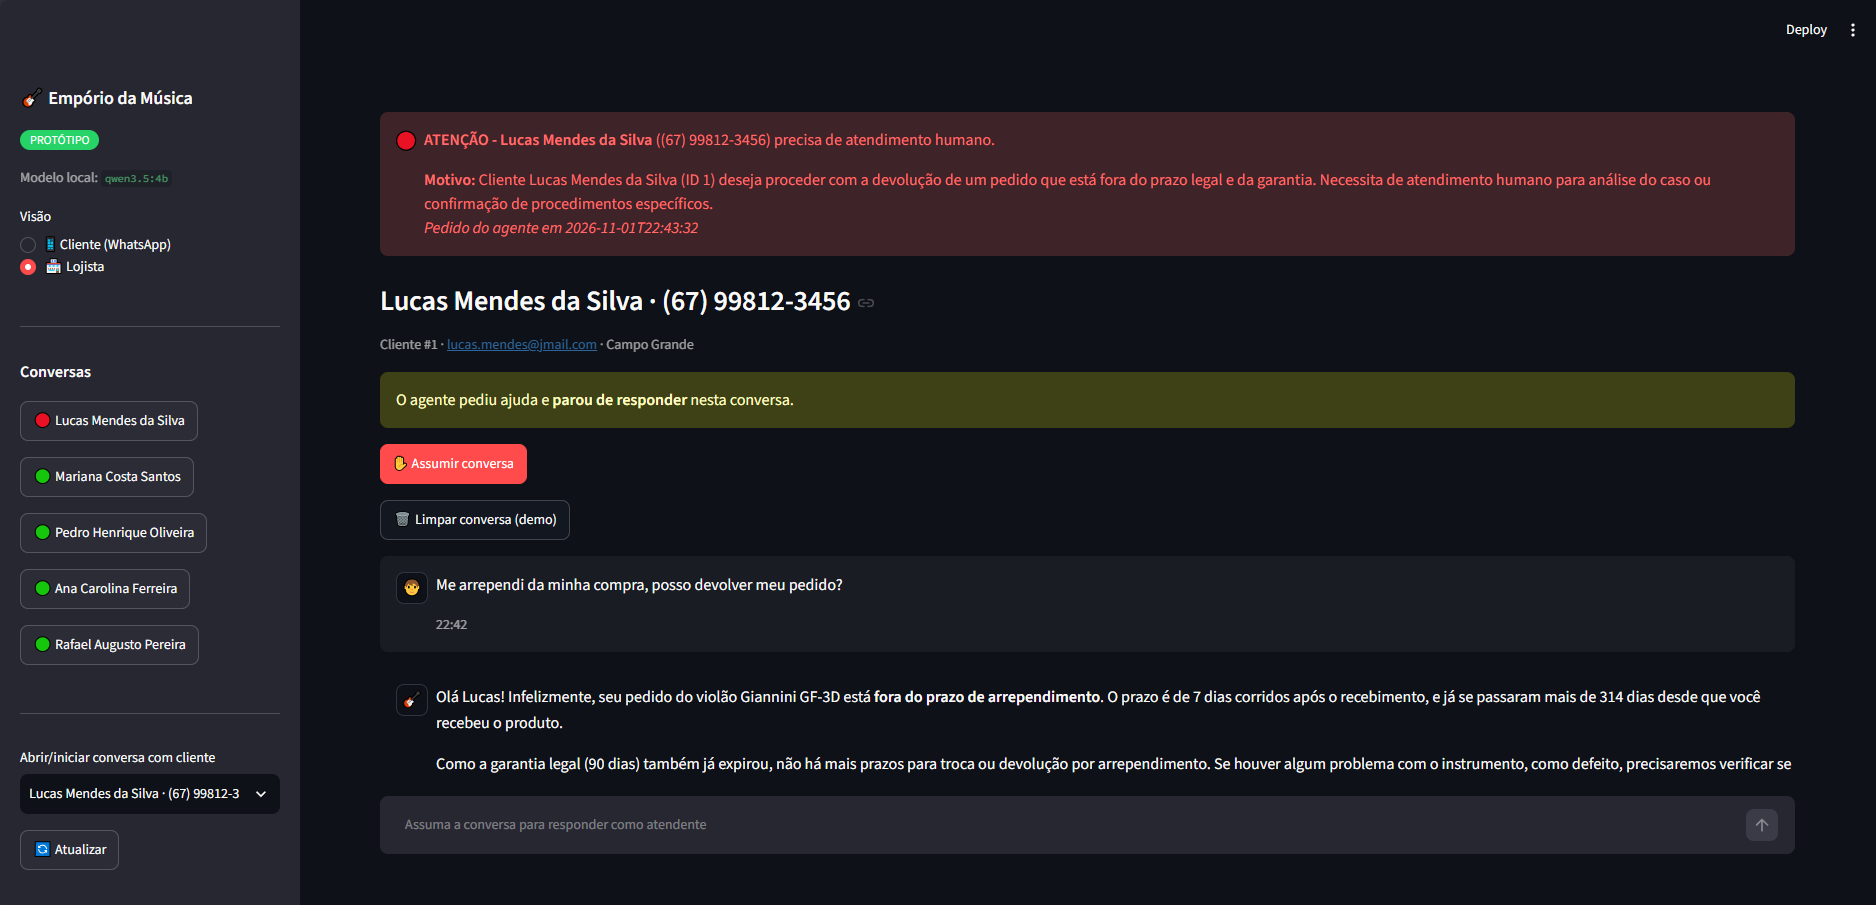
\includegraphics[width=0.45\textwidth]{imgs/print_lucas.png} &
    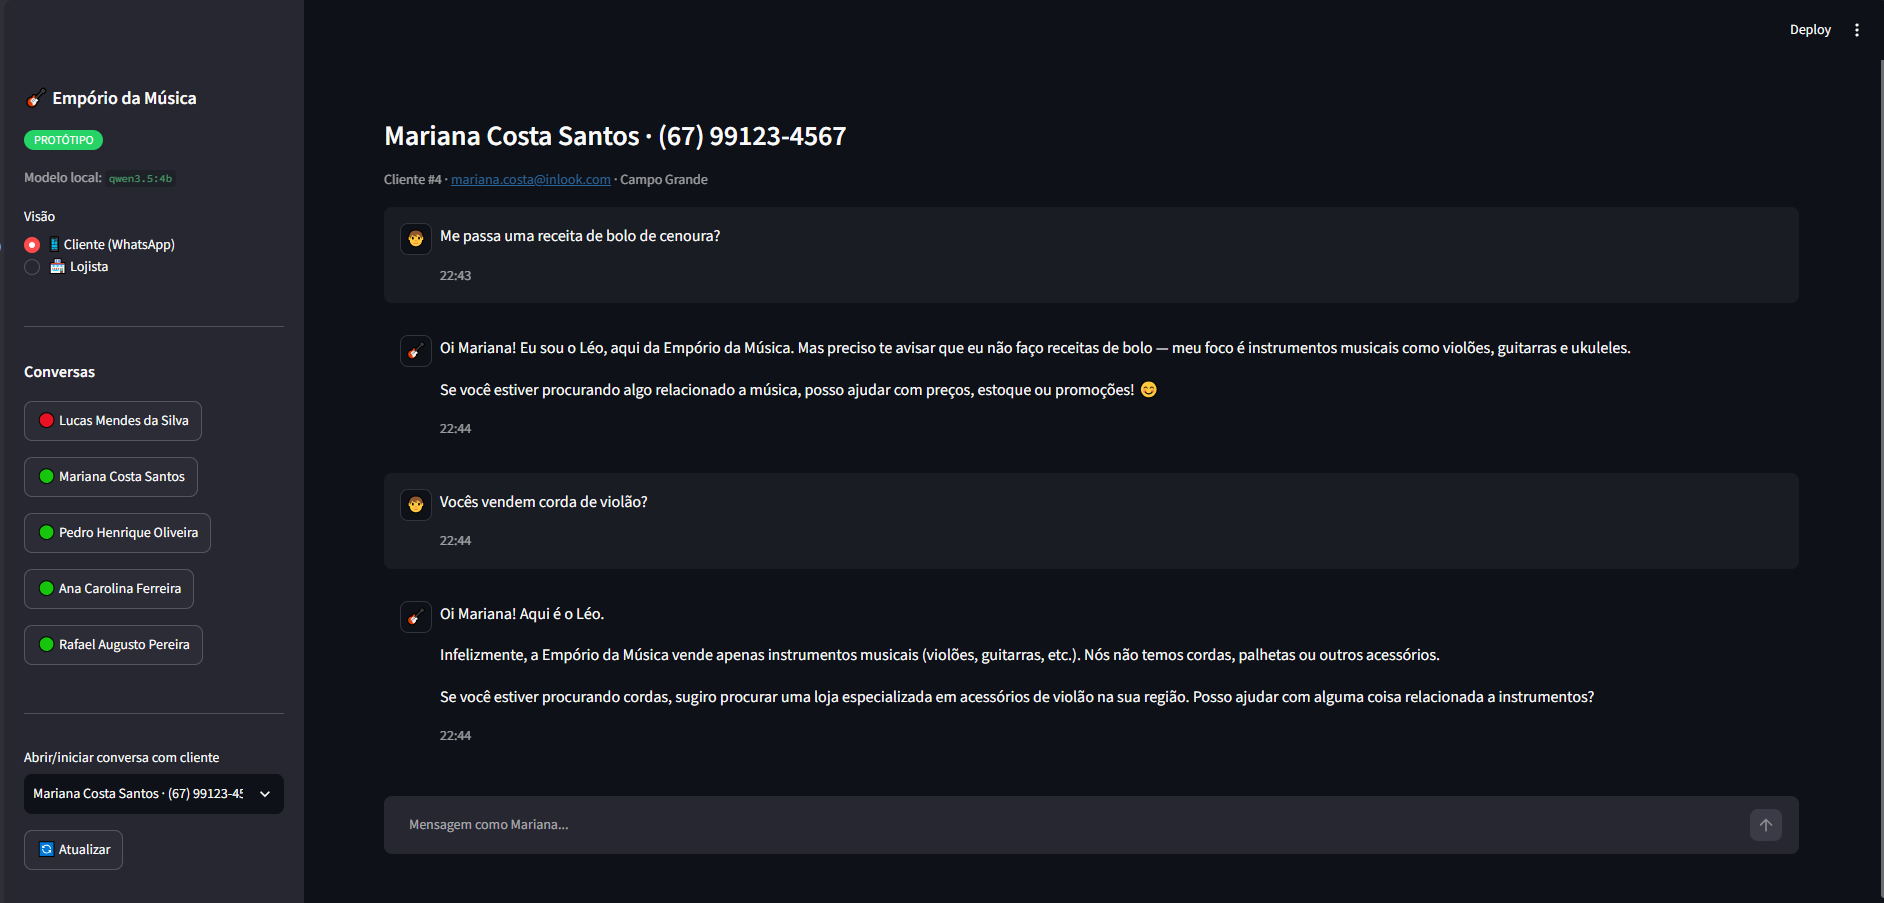
\includegraphics[width=0.45\textwidth]{imgs/print_mariana.png} \\
    \footnotesize\textbf{(a) Shopkeeper View:} Red alert banner \& MCP trace &
    \footnotesize\textbf{(b) Customer View:} Scope refusal \& redirection
\end{tabular}
\end{center}

\subsection{Summary of the 16 Evaluated \& Exported Scenarios (\texttt{examples/})}
All 16 scenarios were executed against the live agent (\texttt{python -m evals.run\_scenarios --export}) and passed (\textbf{16/16 PASS}). Each exported Markdown file records the \textbf{processing time per turn}, the \textbf{exact Python tool call signature}, the \textbf{JSON arguments sent}, and the \textbf{full JSON output returned by the MCP server}.

\begingroup
\footnotesize
\setlength{\tabcolsep}{3.5pt}
\begin{longtable}{c >{\ttfamily\raggedright\arraybackslash}p{3.5cm} >{\raggedright\arraybackslash}p{3.8cm} >{\raggedright\arraybackslash}p{6.5cm} r}
\toprule
\textbf{\#} & \textbf{\normalfont\bfseries File} & \textbf{Scenario} & \textbf{MCP Tools Verified \& Highlights} & \textbf{Time} \\
\midrule
\endfirsthead
\toprule
\textbf{\#} & \textbf{\normalfont\bfseries File} & \textbf{Scenario} & \textbf{MCP Tools Verified \& Highlights} & \textbf{Time} \\
\midrule
\endhead
01 & 01\_catalogo.md & Guitars up to R\$ 1000 + Yamaha C40 details & \texttt{search\_products} (\texttt{max\_price=1000}) $\rightarrow$ \texttt{get\_product\_details} (\texttt{'Yamaha C40'}) & 122.3s \\
\addlinespace[2pt]
02 & 02\_loja.md & Store address + ``Are you open right now?'' & \texttt{get\_store\_policies} (\texttt{'about\_and\_contact'}) $\rightarrow$ \texttt{get\_opening\_status()} & 72.5s \\
\addlinespace[2pt]
03 & 03\_preco\_\allowbreak promocao.md & Takamine GD20 price + active promotions & \texttt{get\_product\_details} (\texttt{'Takamine GD20'}) $\rightarrow$ \texttt{search\_products} (\texttt{on\_promotion=True}) & 53.7s \\
\addlinespace[2pt]
04 & 04\_devolucao.md & \textbf{Non-trivial:} Regret return on delivered order & \texttt{get\_customer\_orders} (\texttt{customer\_id=1}, 315 days $>$ 7-day limit) $\rightarrow$ \texttt{request\_human\_handoff} & 95.0s \\
\addlinespace[2pt]
05 & 05\_fora\_escopo.md & Carrot cake recipe + guitar strings request & Direct polite refusal for out-of-scope \& accessory redirection (no tools called) & 58.3s \\
\addlinespace[2pt]
06 & 06\_produto\_\newline esgotado.md & Out-of-stock Giannini GF-3D & \texttt{get\_product\_details} (\texttt{'Giannini GF-3D'}) $\rightarrow$ stock 0 + suggests 3 available alternatives & 48.2s \\
\addlinespace[2pt]
07 & 07\_produto\_\newline descontinuado.md & Discontinued 7-string Shelby SN-7C & \texttt{get\_product\_details} (\texttt{'Shelby SN-7C'}) $\rightarrow$ informs discontinued status + alternatives & 51.2s \\
\addlinespace[2pt]
08 & 08\_pix\_nao\_\newline cumulativo.md & Crafter HT-100 promo + PIX discount question & \texttt{get\_product\_details} (\texttt{'Crafter HT-100'}) $\rightarrow$ shows 18\% promo \& explains 5\% PIX does not stack & 51.0s \\
\addlinespace[2pt]
09 & 09\_rastreio\_\newline pedido.md & Order \#8 status \& tracking code & \texttt{get\_customer\_orders} (\texttt{customer\_id=2}, \texttt{order\_id='8'}) $\rightarrow$ \texttt{shipped}, \texttt{BRJL5544332BR} & 65.2s \\
\addlinespace[2pt]
10 & 10\_pedido\_\newline cancelado.md & Why was my order cancelled? & \texttt{get\_customer\_orders} (\texttt{customer\_id=17}) $\rightarrow$ reads cancellation \texttt{notes} (item out of stock) & 46.5s \\
\addlinespace[2pt]
11 & 11\_parcelamento\_e\_\newline entrega\_sp.md & \textbf{Multi-turn:} Credit card installments + shipping to S\~ao Paulo & Turn 1: \texttt{get\_store\_policies} (\texttt{'payment'}, up to 12x rules) $\rightarrow$ Turn 2: \texttt{get\_store\_policies} (\texttt{'shipping'}, Correios/Jadlog deadlines) & 172.4s \\
\addlinespace[2pt]
12 & 12\_frete\_entrega.md & Shipping to Campo Grande vs.\ other cities & \texttt{get\_store\_policies} (\texttt{'shipping'}) $\rightarrow$ motoboy (free $>$ R\$ 500) vs.\ PAC, SEDEX, Jadlog & 54.1s \\
\addlinespace[2pt]
13 & 13\_garantia.md & Warranty rules + broken string question & \texttt{get\_store\_policies} (\texttt{'warranty'}) $\rightarrow$ 90-day legal + manufacturer warranty; broken strings excluded & 52.9s \\
\addlinespace[2pt]
14 & 14\_categorias.md & Product categories sold by the store & \texttt{list\_categories()} $\rightarrow$ lists active instrument categories and counts & 49.1s \\
\addlinespace[2pt]
15 & 15\_reclamacao\_\newline handoff.md & Warped guitar neck complaint & Empathy + escalates immediately via \texttt{request\_human\_handoff} (red alert) & 32.3s \\
\addlinespace[2pt]
16 & 16\_entrada\_\newline aleatoria.md & \textbf{Gibberish input} (\texttt{askdjansdkj}) + recovery & Turn 1: asks for clarification without calling tools $\rightarrow$ Turn 2: \texttt{search\_products} (\texttt{'violao nylon'}, \texttt{max\_price=700}) & 110.6s \\
\bottomrule
\end{longtable}
\endgroup

\subsection{Sample Rich Trace Excerpt (from \texttt{examples/04\_devolucao.md})}
Below is an excerpt illustrating how the exported \texttt{.md} files document both the agent's exact function call and the MCP server's response:

\begin{lstlisting}
### Turno 1 (Scenario 04 - Return Request)
Cliente (Lucas): Me arrependi da minha compra, posso devolver meu pedido?
Leo (55.55s): Ola Lucas! Infelizmente, seu pedido do violao Giannini GF-3D ja esta *fora do prazo de arrependimento* (7 dias corridos apos o recebimento)... Quer que eu encaminhe para um atendente humano?

1. Chamada realizada pelo agente:
   get_customer_orders(customer_id=1)
Resposta obtida da funcao (MCP / Tool Output):
   { "found": true, "today": "2026-11-02",
     "orders": [{ "order_id": 4, "status": "delivered", "estimated_delivery": "2025-12-22",
       "policy_check": { "days_since_receipt_approx": 315,
         "regret_return_7_days": "FORA do prazo (7 dias corridos apos o recebimento)",
         "legal_warranty_90_days": "expirada" } }] }

### Turno 2 (Scenario 04 - Handoff Confirmation)
Cliente (Lucas): Sim, quero devolver.
1. Chamada realizada pelo agente:
   request_human_handoff(reason='Cliente Lucas Mendes da Silva (customer_id=1) deseja prosseguir com a devolucao de um pedido, mas o prazo legal de arrependimento ja expirou...')
-> RED ALERT triggered on Shopkeeper Dashboard (mode = waiting_human)
\end{lstlisting}

% ------------------------------------------------------------------ 6. LIMITATIONS
\section{Known Limitations \& Future Improvements}
\label{sec:limitations}

\textbf{Known Limitations}
\begin{itemize}
    \item \textbf{Simulated WhatsApp UI:} Streamlit is used for rapid prototyping; there is no live webhook to the WhatsApp Business Cloud API yet, and the shopkeeper dashboard requires a manual refresh.
    \item \textbf{Local Hardware Latency:} Running a 4B/9B model on a 4 GB GTX 1650 yields 25--60s latency per turn without token streaming.
    \item \textbf{Small Model Quirks:} A 4B model can occasionally omit items from a list or skip a tool call in multi-turn conversations. This is mitigated via deterministic Python calculations and runtime retry guard rails, but not 100\% eliminated.
    \item \textbf{Receipt Date Proxy:} \texttt{orders.csv} only provides \texttt{estimated\_delivery}, which is used as a proxy for the delivery date when computing the 7-day regret window (flagged in \texttt{policy\_check.obs}).
    \item \textbf{Phone vs.\ WhatsApp Distinction:} The manual lists two numbers; as clarified in the business rules, \texttt{(67) 3341-4444} is for voice calls only and \texttt{(67) 3321-4500} is exclusively for WhatsApp messages.
\end{itemize}

\textbf{What Would Be Done With More Time}
\begin{itemize}
    \item \textbf{FastAPI + WebSocket Frontend \& WhatsApp Webhook:} Replace Streamlit with a FastAPI backend pushing real-time WebSocket alerts to multiple authenticated shopkeepers and connecting directly to the WhatsApp Business API.
    \item \textbf{Multi-Agent Architecture (A2A):} Evolve into specialized agents communicating via A2A (e.g., Catalog/Sales Advisor, Post-Sale \& Logistics Agent, Billing Agent) once new external integrations are added.
    \item \textbf{LangGraph Stateful Flows:} Use LangGraph for guided multi-step workflows (e.g., collecting defect photos and serial numbers before human handoff) and human-approved write tools.
    \item \textbf{Production Inference \& Observability:} Deploy on a dedicated GPU / vLLM or hosted API for $<3$s latency with token streaming, semantic caching for FAQs, and Langfuse/LangSmith tracing + LLM-as-a-judge evaluations.
\end{itemize}

% ------------------------------------------------------------------ 7. AI ASSISTANTS & REPO STRUCTURE
\section{Use of AI Coding Assistants \& Repository Structure}

\textbf{Workflow with AI Coding Assistant:} This project was developed using \textbf{Antigravity} (Google DeepMind's agentic coding assistant) in a pair-programming workflow:
\begin{enumerate}
    \item \textbf{Problem Framing \& Architecture (Human):} I defined the core architecture: local Ollama model for zero cost/privacy, MCP server for data/policy tools, A2A reserved for multi-agent evolution, WhatsApp-like UI populated from \texttt{customers.csv}, and autonomous operation with a red alert human handoff for the shopkeeper.
    \item \textbf{Data Exploration \& Planning:} The assistant inspected all CSVs and the policy PDF, surfacing key edge cases (only 4 of 25 promotions active, non-cumulative PIX discount, no accessories sold, all delivered orders past the 7-day regret window) in an implementation plan.
    \item \textbf{Technical Decisions (Human):} I reviewed the plan and chose LangChain, Streamlit as an explicit prototype (with FastAPI documented as future work), English tool schemas with strict Portuguese responses, and versioning \texttt{data/}.
    \item \textbf{Incremental Implementation \& Empirical Tuning:} Built in small commits with deterministic \texttt{pytest} tests first. When benchmarking showed \texttt{qwen3.5:9b} took $\sim$3.5 min/turn on my GPU, I decided to switch the default to \texttt{qwen3.5:4b} ($\sim$2x faster) and added runtime guard rails after observing multi-turn tool-calling edge cases.
\end{enumerate}

\textbf{Repository Structure:}
\begin{lstlisting}
app/
  agent/            agent.py (LangChain + MCP + Ollama + guard rails), prompts.py
  mcp_server/       server.py (FastMCP tools over stdio)
  knowledge/        politicas.md (curated store manual by topic)
  storage/          chat_store.py (SQLite threads, messages, tool traces & mode)
  ui/               streamlit_app.py (WhatsApp customer view + Shopkeeper alert panel)
  repository.py     SQLite queries + deterministic business rules (promo/PIX/returns)
  ingest.py         CSV -> SQLite loader
  config.py, cli.py Configuration & terminal chat CLI
data/               Store CSVs and policies PDF provided by the challenge
tests/              16 deterministic pytest unit tests (no LLM required)
evals/              run_scenarios.py (16 end-to-end evals + rich Markdown exporter)
examples/           16 exported real conversations with full MCP JSON traces & timing
imgs/               UI screenshots (Shopkeeper red alert & Customer chat)
\end{lstlisting}

\end{document}
